\documentclass[10pt]{beamer}

\usetheme[progressbar=frametitle]{metropolis}
\usepackage{appendixnumberbeamer}
\usepackage{booktabs}
\usepackage[scale=2]{ccicons}
\usepackage{pgfplots}
\usepgfplotslibrary{dateplot}
\usepackage{xspace}
\usepackage{algorithm}
\usepackage{algpseudocode}
\usepackage{amsmath, amssymb}
\usepackage{graphicx}
\usepackage{subcaption}
\usepackage{hyperref}
\usepackage{multirow}

\newcommand{\themename}{\textbf{\textsc{metropolis}}\xspace}
\newcommand{\w}{\vec{\textbf{w}}}
\newcommand{\costder}{\frac{\partial MSE}{\partial w_j}(\w)}
\newcommand{\R}{\mathbb{R}}

\title{Machine Learning - Exercise 3}
\subtitle{Model Stealing/Extraction}
% \date{\today}
\date{}
\author{Esra Ceylan, Daniel Fangl, Christian Hatschka}
\institute{TU Wien}
% \titlegraphic{\hfill\includegraphics[height=1.5cm]{logo.pdf}}

\begin{document}
\maketitle
\begin{frame}{Table of contents}
  \setbeamertemplate{section in toc}[sections numbered]
  \tableofcontents%[hideallsubsections]
\end{frame}
\section[Copy-Cat Stealing]{Copy-Cat Stealing}
\begin{frame}[fragile]{Basics}
\begin{itemize}
    \item Uses model as blackbox
    \item unlabeled images (domain + non-domain)
    \item Stochastic Gradient Descent with a Step Down policy for learning rate
\end{itemize}
\end{frame}
\subsection[Microsoft Azure API]{Microsoft Azure API}

\begin{frame}[fragile]{Azure API}
\begin{itemize}
    \item Gives a percentage vector of emotions (Anger, Contempt, Disgust, Fear, Happiness, Neutral, Sadness, Surprise)
    \item No such vector if it doesn't recognise a face$\Rightarrow$Only domain data
    \item Free to use but has premium plan
\end{itemize}
\end{frame}
\begin{frame}[fragile]{The dataset}
\noindent\begin{minipage}{\textwidth}% adapt widths of minipages to your needs
\begin{itemize}
\item KDEF and AKDEF 
\item Emotion Detection from Facial Expressions
\item contains already labeled data
\end{itemize}
\end{minipage}

 \begin{figure}[h!]
        \centering
        \begin{subfigure}[c]{0.45\textwidth}
            \centering
            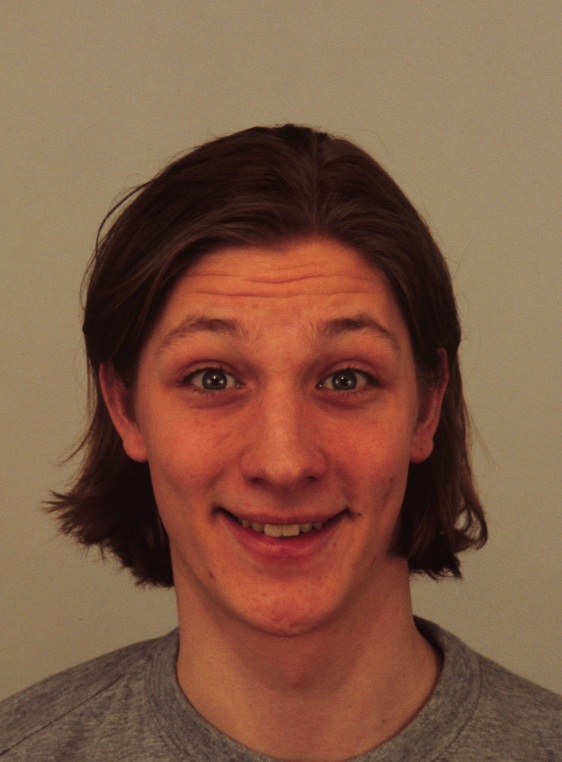
\includegraphics[width=0.9\textwidth]{exercise_3/paper/images/AM18HAS.JPG}
            \caption{A face from KDEF}
            \label{fig:KDEF_face}
        \end{subfigure}
        \begin{subfigure}[c]{0.45\textwidth}
            \centering
            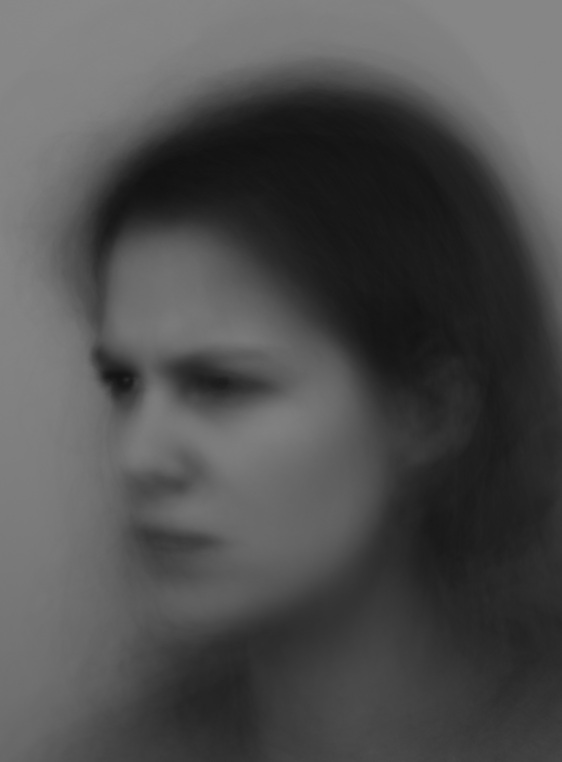
\includegraphics[width=0.9\textwidth]{exercise_3/paper/images/FANHL.JPG}
            \caption{A face from AKDEF}
            \label{fig:AKDEF_face}
        \end{subfigure}
        \caption{}
        \label{fig:faces}
    \end{figure}
\end{frame}
\begin{frame}[fragile]{Evaluation}
\begin{itemize}
    \item Accuracy of Azure on labeled data roughly $0.76$
    \item attack set: starting with $2000$ up to $13961$
    \item Test set: $4654$
    \item one hour including queries
\end{itemize}
\end{frame}
\begin{frame}[fragile]{Evaluation}
           \begin{figure}[h!]
                    \centering      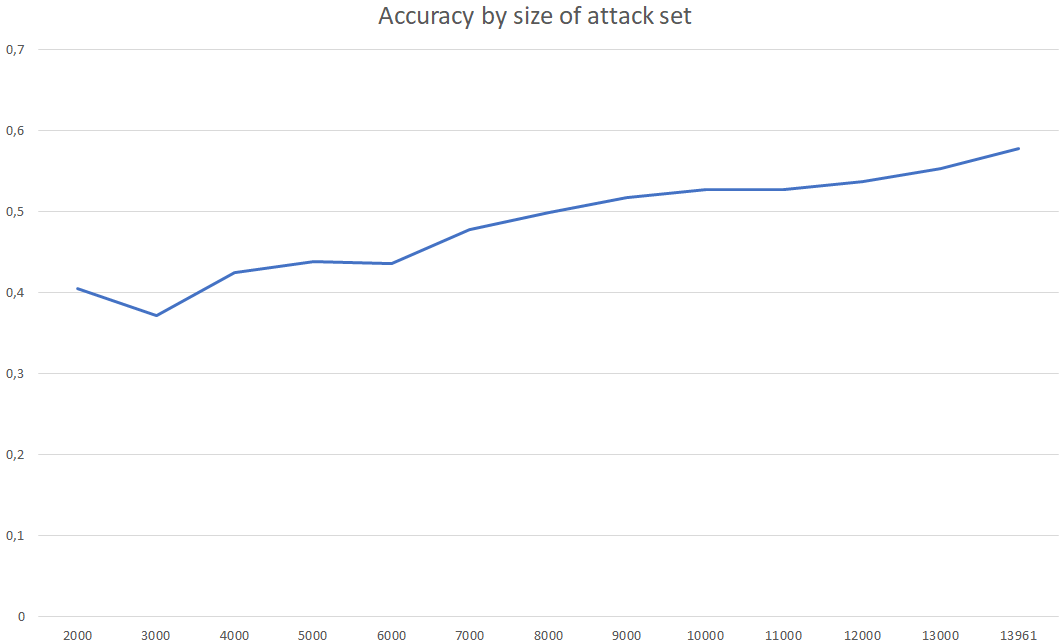
\includegraphics[scale=0.8]{exercise_3/paper/images/accuracy_copy_Azure.png}
                    \caption{Accuracy of the copied network}
                    \label{fig:Ac_Azure}
            \end{figure}
        
\end{frame}
\begin{frame}[fragile]{Evaluation}
           \begin{figure}[h!]
                    \centering      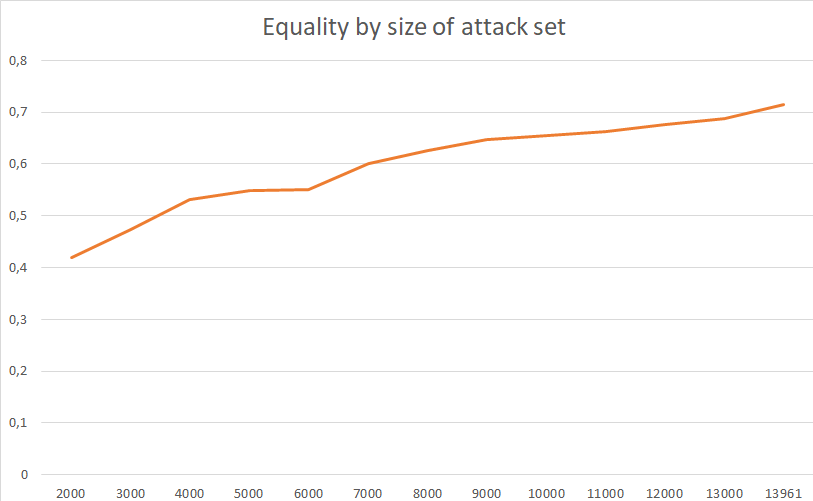
\includegraphics[scale=0.8]{exercise_3/paper/images/equality_copy_Azure.png}
                    \caption{percentage of images labeled the same}
                    \label{fig:Eq_AZure}
            \end{figure}
        
\end{frame}
\subsection[Cats and dogs]{Cats and dogs}
\begin{frame}[fragile]{Cats and dogs Model}
\begin{itemize}
\item CNN home trained on $25\,000$ images
\item Accuracy: $0,821$
\end{itemize}
\end{frame}
\begin{frame}[fragile]{Evaluation}
                \begin{figure}[h!]
            \centering
            \begin{subfigure}[c]{0.49\textwidth}
                \centering
                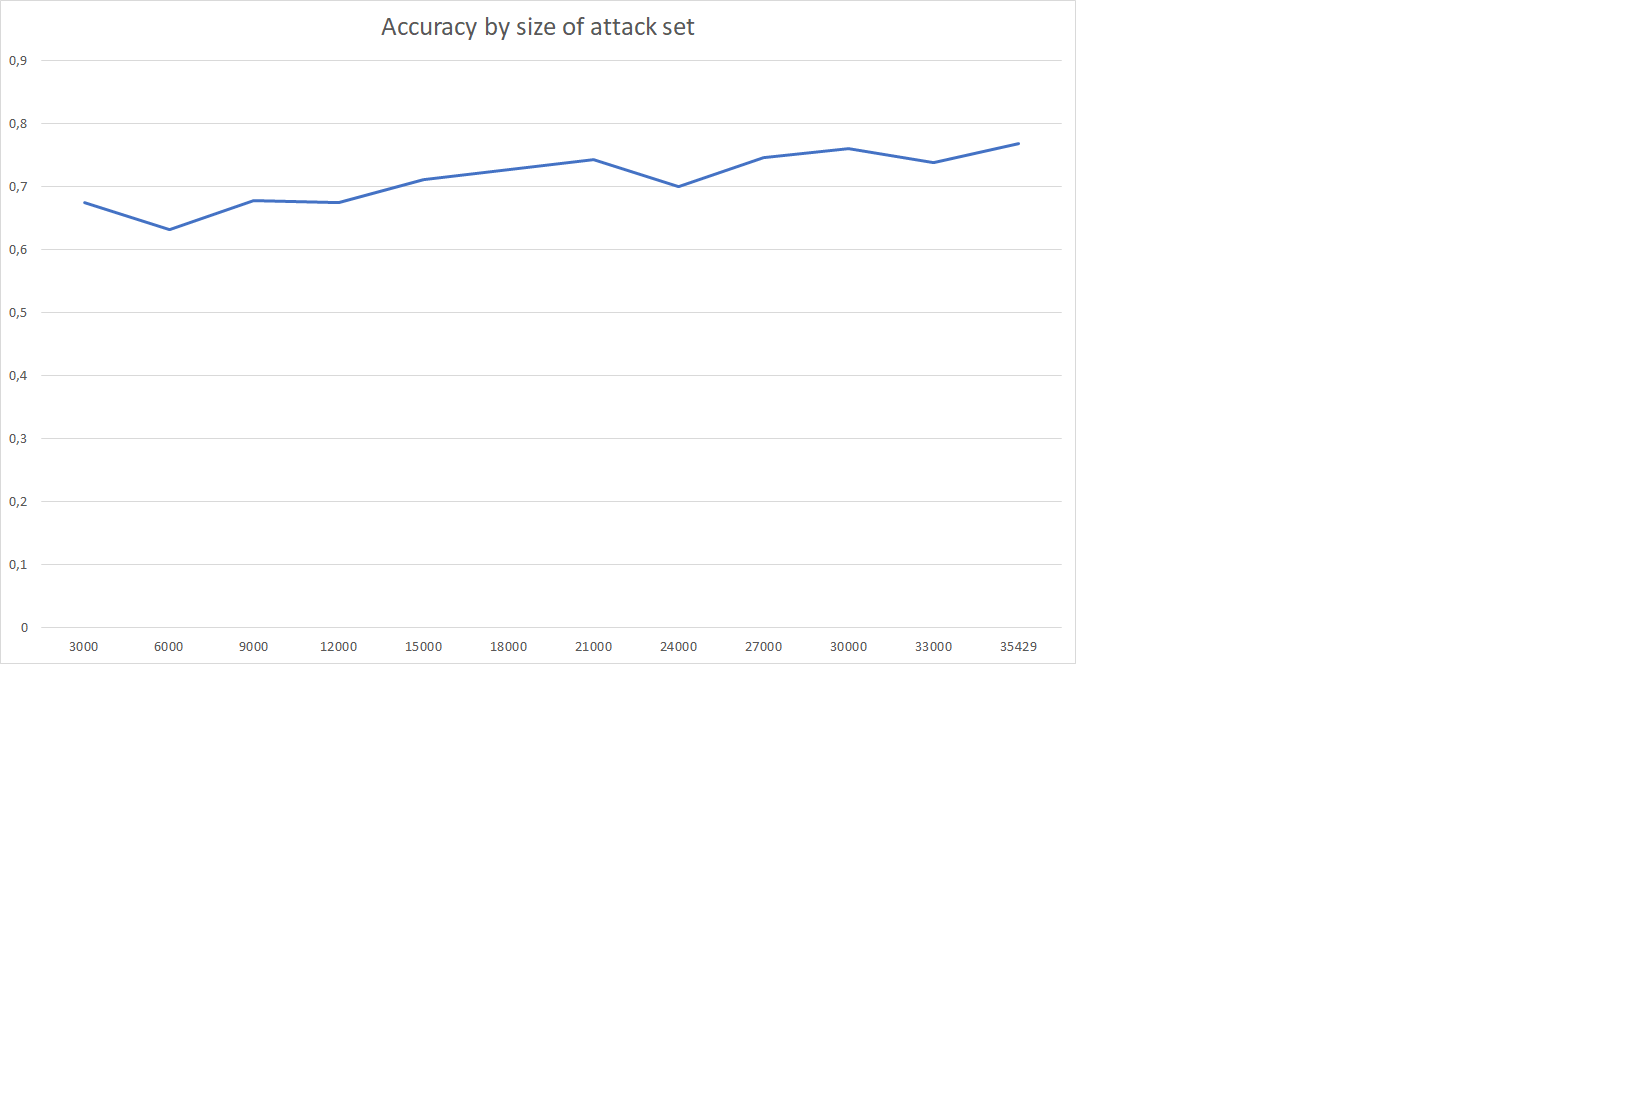
\includegraphics[width=1\textwidth]{exercise_3/paper/images/Accuracy_copy_cat_domain.png}
                \caption{Accuracy using only problem domain}
                \label{fig:Accuracy_Cat_domain}
            \end{subfigure}
            \begin{subfigure}[c]{0.49\textwidth}
                \centering
                \includegraphics[width=1\textwidth]{exercise_3/paper/images/Accuracy_copy_cat.png}
                \caption{Accuracy using mixed instances }
                \label{fig:Accuracy_cat_mix}
            \end{subfigure}
            \caption{Accuracy of Copycat Attack on second data set}
            \label{fig:accuracy_cat}
        \end{figure}
\end{frame}
\begin{frame}[fragile]{Evaluation}
       \begin{figure}[h!]
            \centering
            \begin{subfigure}[c]{0.49\textwidth}
                \centering
                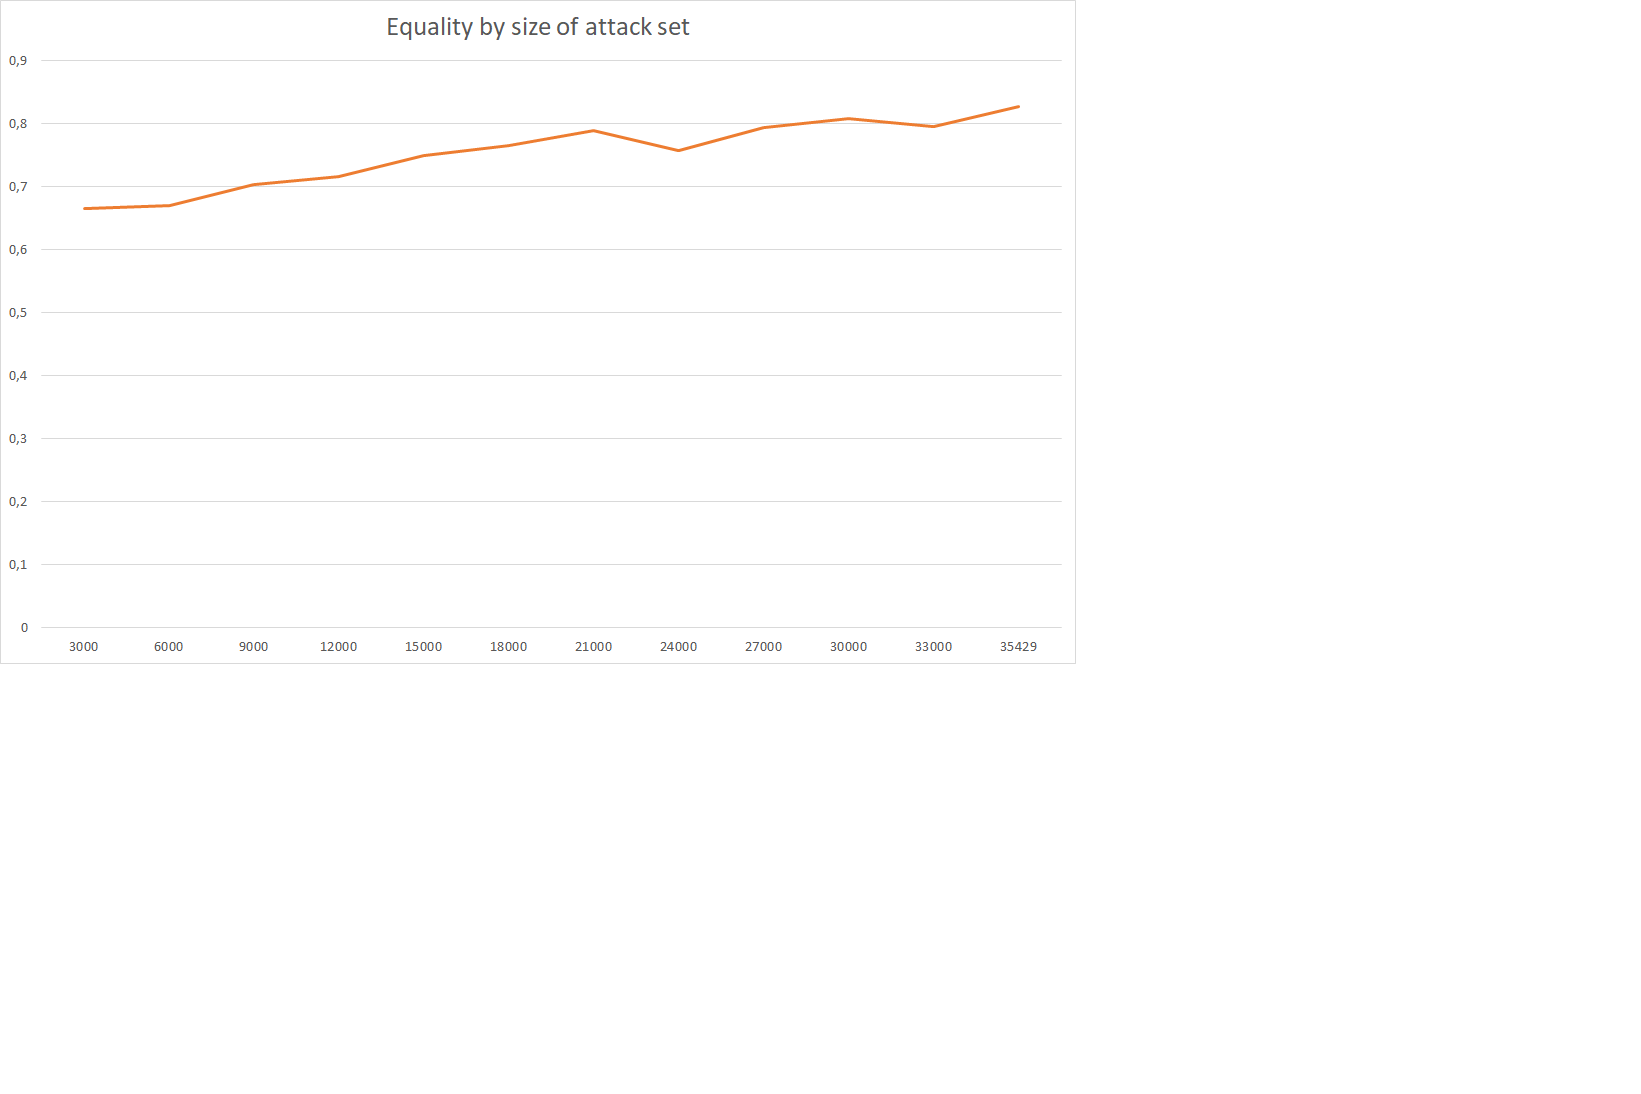
\includegraphics[width=1\textwidth]{exercise_3/paper/images/Equality_copy_cat_domain.png}
                \caption{Equality using only problem domain}
                \label{fig:Equality_cat_domain}
            \end{subfigure}
            \begin{subfigure}[c]{0.49\textwidth}
                \centering
                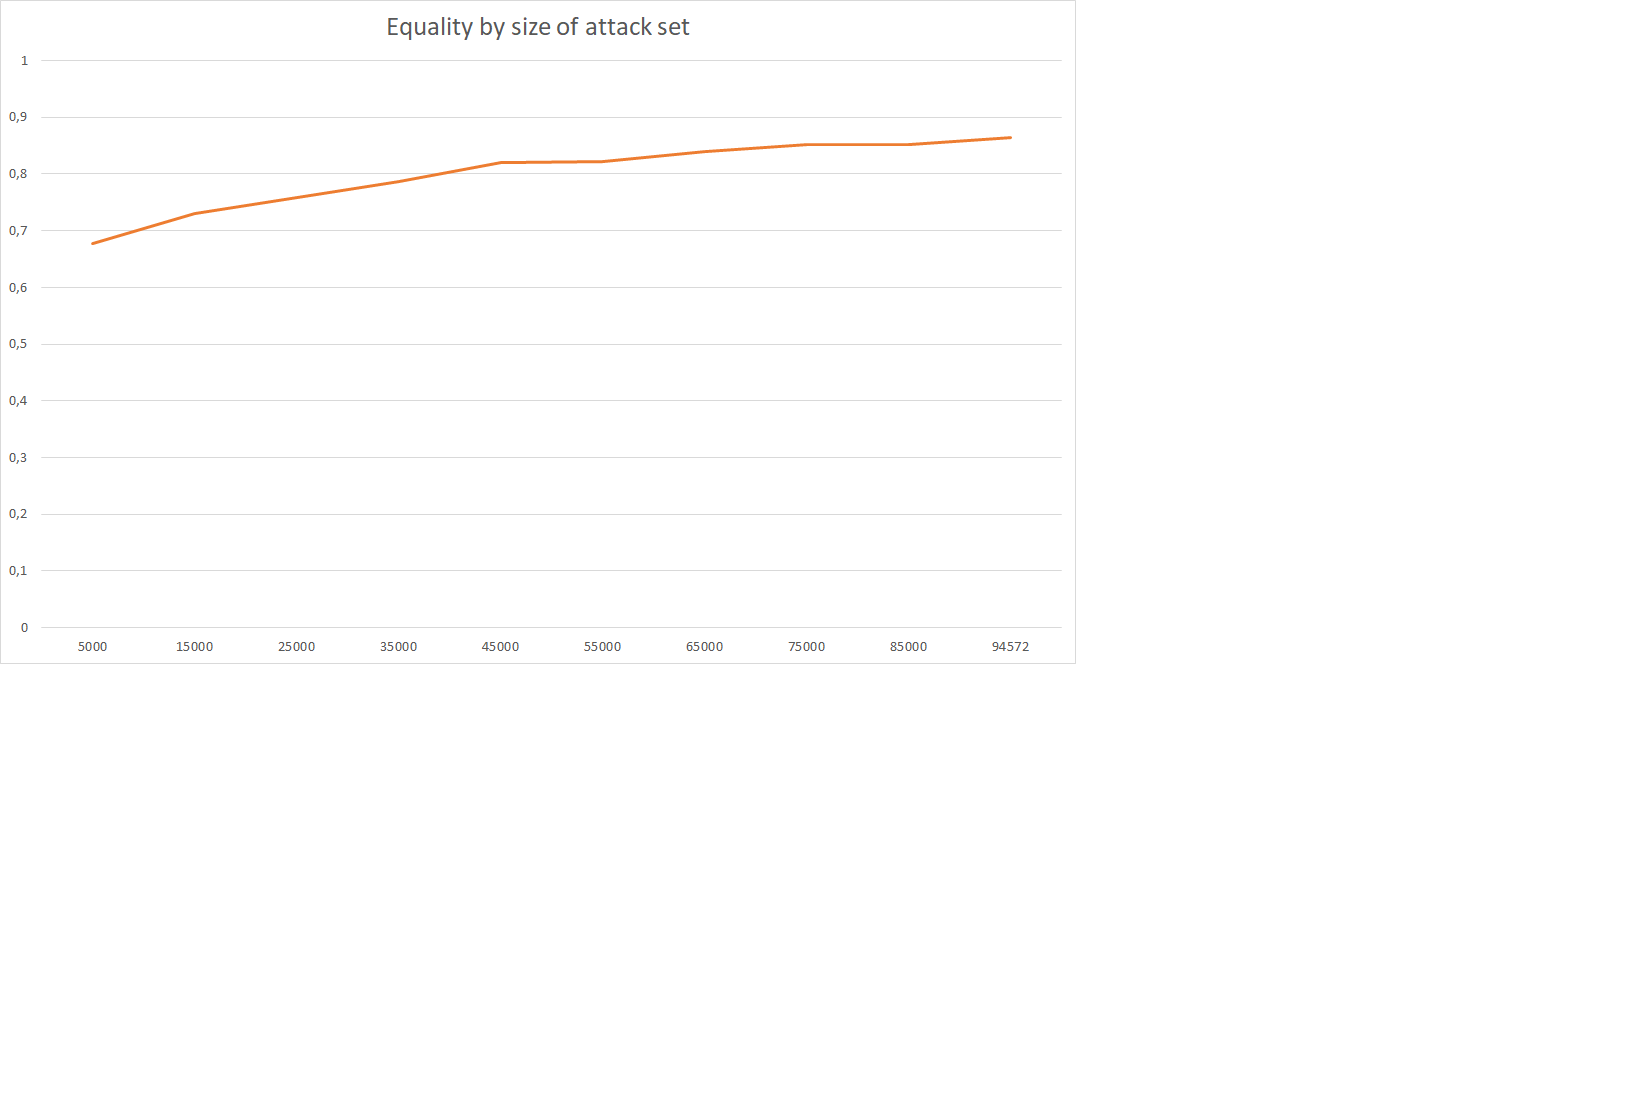
\includegraphics[width=1\textwidth]{exercise_3/paper/images/Equality_copy_cat.png}
                \caption{Equality using mixed instances}
                \label{fig:Equality_cat_mix}
            \end{subfigure}
            \caption{Equality of Copycat Attack on second data set}
            \label{fig:equality_cat}
        \end{figure}
\end{frame}
\begin{frame}[fragile]{runtime}
    \begin{figure}[h!]
        \centering      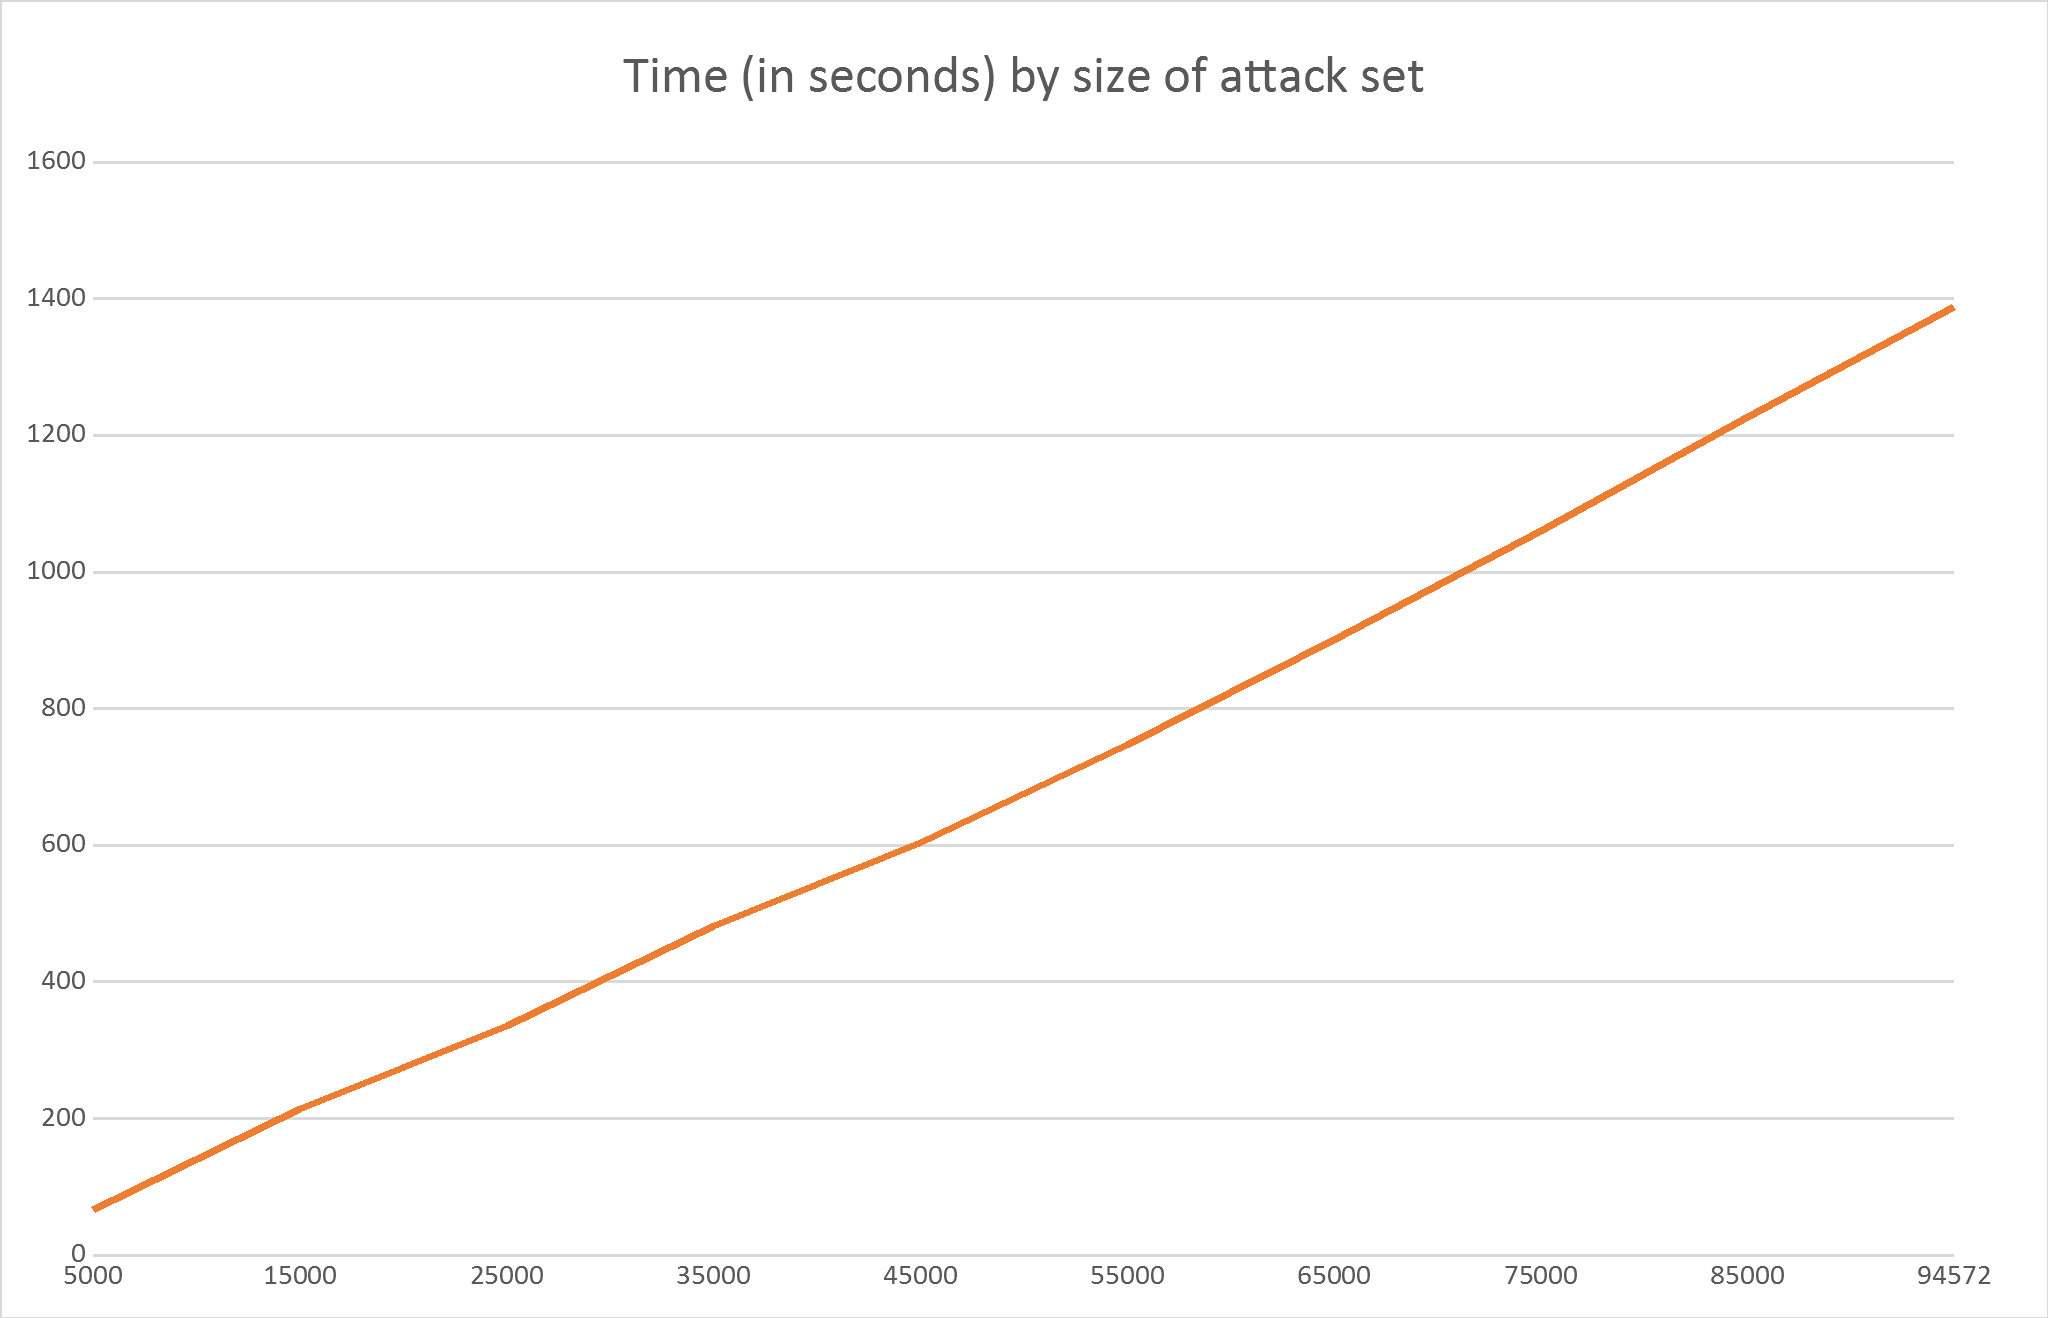
\includegraphics[scale=0.4]{exercise_3/paper/images/Time_copy_cat.png}
        \caption{Time needed to extract a model}
        \label{fig:time_cat}
    \end{figure}
\end{frame}

\end{document}
